\documentclass[uplatex,dvipdfmx]{jlreq}
\usepackage[fleqn,tbtags]{mathtools}
\usepackage{jlreq-deluxe}
\usepackage{geometry}
\usepackage{booktabs}
\usepackage{hyperref}
\usepackage[noalphabet]{pxchfon} % must be after otf package
\usepackage{stix2} %欧文＆数式フォント
\usepackage[fleqn,tbtags]{mathtools} % 数式関連 (w/ amsmath)
\usepackage{url}
\usepackage{here}
\geometry{left=20mm,right=20mm,top=25mm,bottom=25mm}

\title{作業ログ\\ \large 加速度センサーを用いた身体動作による輪唱制御システムの構築と視覚フィードバック効果}
\author{報告者: 早川　和輝}
\date{報告日: 2026年7月1日}

\begin{document}
\maketitle

\section{進捗サマリー(要約)}
\begin{itemize}
    \item 全体進捗率: [95\%]
    \item マイルストーン達成状況: [達成]
    \item 主要成果:
    \begin{itemize}
        \item 成果1: 制御用Arduinoと同期用Arduinoのコマンド連携を統合し，無線コマンドで全楽器の再生・輪唱・テンポ変更を制御できることを確認．
        \item 成果2: バイオリン・ギロを含む楽器Arduino4台とサーボ・LEDマトリクスを統合し，実機での動作確認を実施．4台が輪唱として連動して動作することを確認した．
        \item 成果3: 音とLEDマトリクス(カエルのアニメーション)の同期確認を行い，再生・テンポ変更時の音と表示のずれが許容範囲に収まることを確認した．
    \end{itemize}
    \item 重大課題(影響度:無し): なし
\end{itemize}

\section{作業ログ(詳細トラッキング)}
\begin{table}[H]
    \centering
    \small
    \begin{tabular}{lp{1.5cm}p{1.5cm}llp{2.5cm}p{3cm}}
        \toprule
        作業項目 & 開始日 & 完了日 & 状態 & 進捗率 & 依存関係・ブロッカー & コメント \\
        \midrule
        制御・同期の統合 & [6/24] & [6/27] & 完了 & 100\% & なし & 制御用と同期用Arduinoのコマンド連携を統合．無線コマンドで再生・輪唱・テンポ変更を制御． \\
        楽器の統合と動作確認 & [6/25] & [6/29] & 完了 & 100\% & なし & 楽器Arduino4台とサーボ・LEDマトリクスを統合し，実機で4台輪唱の動作を確認． \\
        音とマトリクスの同期確認 & [6/28] & [6/30] & 完了 & 100\% & なし & 音とLEDアニメの同期を確認．再生・テンポ変更時の音ズレが許容範囲に収まることを確認． \\
        \bottomrule
    \end{tabular}
\end{table}

\section{担当箇所の計画前のGCと現在のGC}
担当箇所である「楽器演奏実装」および「統合」における，当初計画時（計画前）のガントチャート（GC）の予定と，現在の進捗・変更状況の比較である．
\begin{table}[H]
    \centering
    \small
    \begin{tabular}{lp{4cm}p{4cm}l}
        \toprule
        タスク名 & 計画前のGC（予定期間） & 現在のGC（実績・修正期間） & 進捗状態 \\
        \midrule
        制御・同期の統合 & [6/22 $\sim$ 6/27] & [6/24 $\sim$ 6/27] & 完了 \\
        楽器の統合と動作確認 & [6/24 $\sim$ 6/29] & [6/25 $\sim$ 6/29] & 完了 \\
        音とマトリクスの同期確認 & [6/27 $\sim$ 6/30] & [6/28 $\sim$ 6/30] & 完了 \\
        \bottomrule
    \end{tabular}
\end{table}\begin{figure}[H]
    \centering
    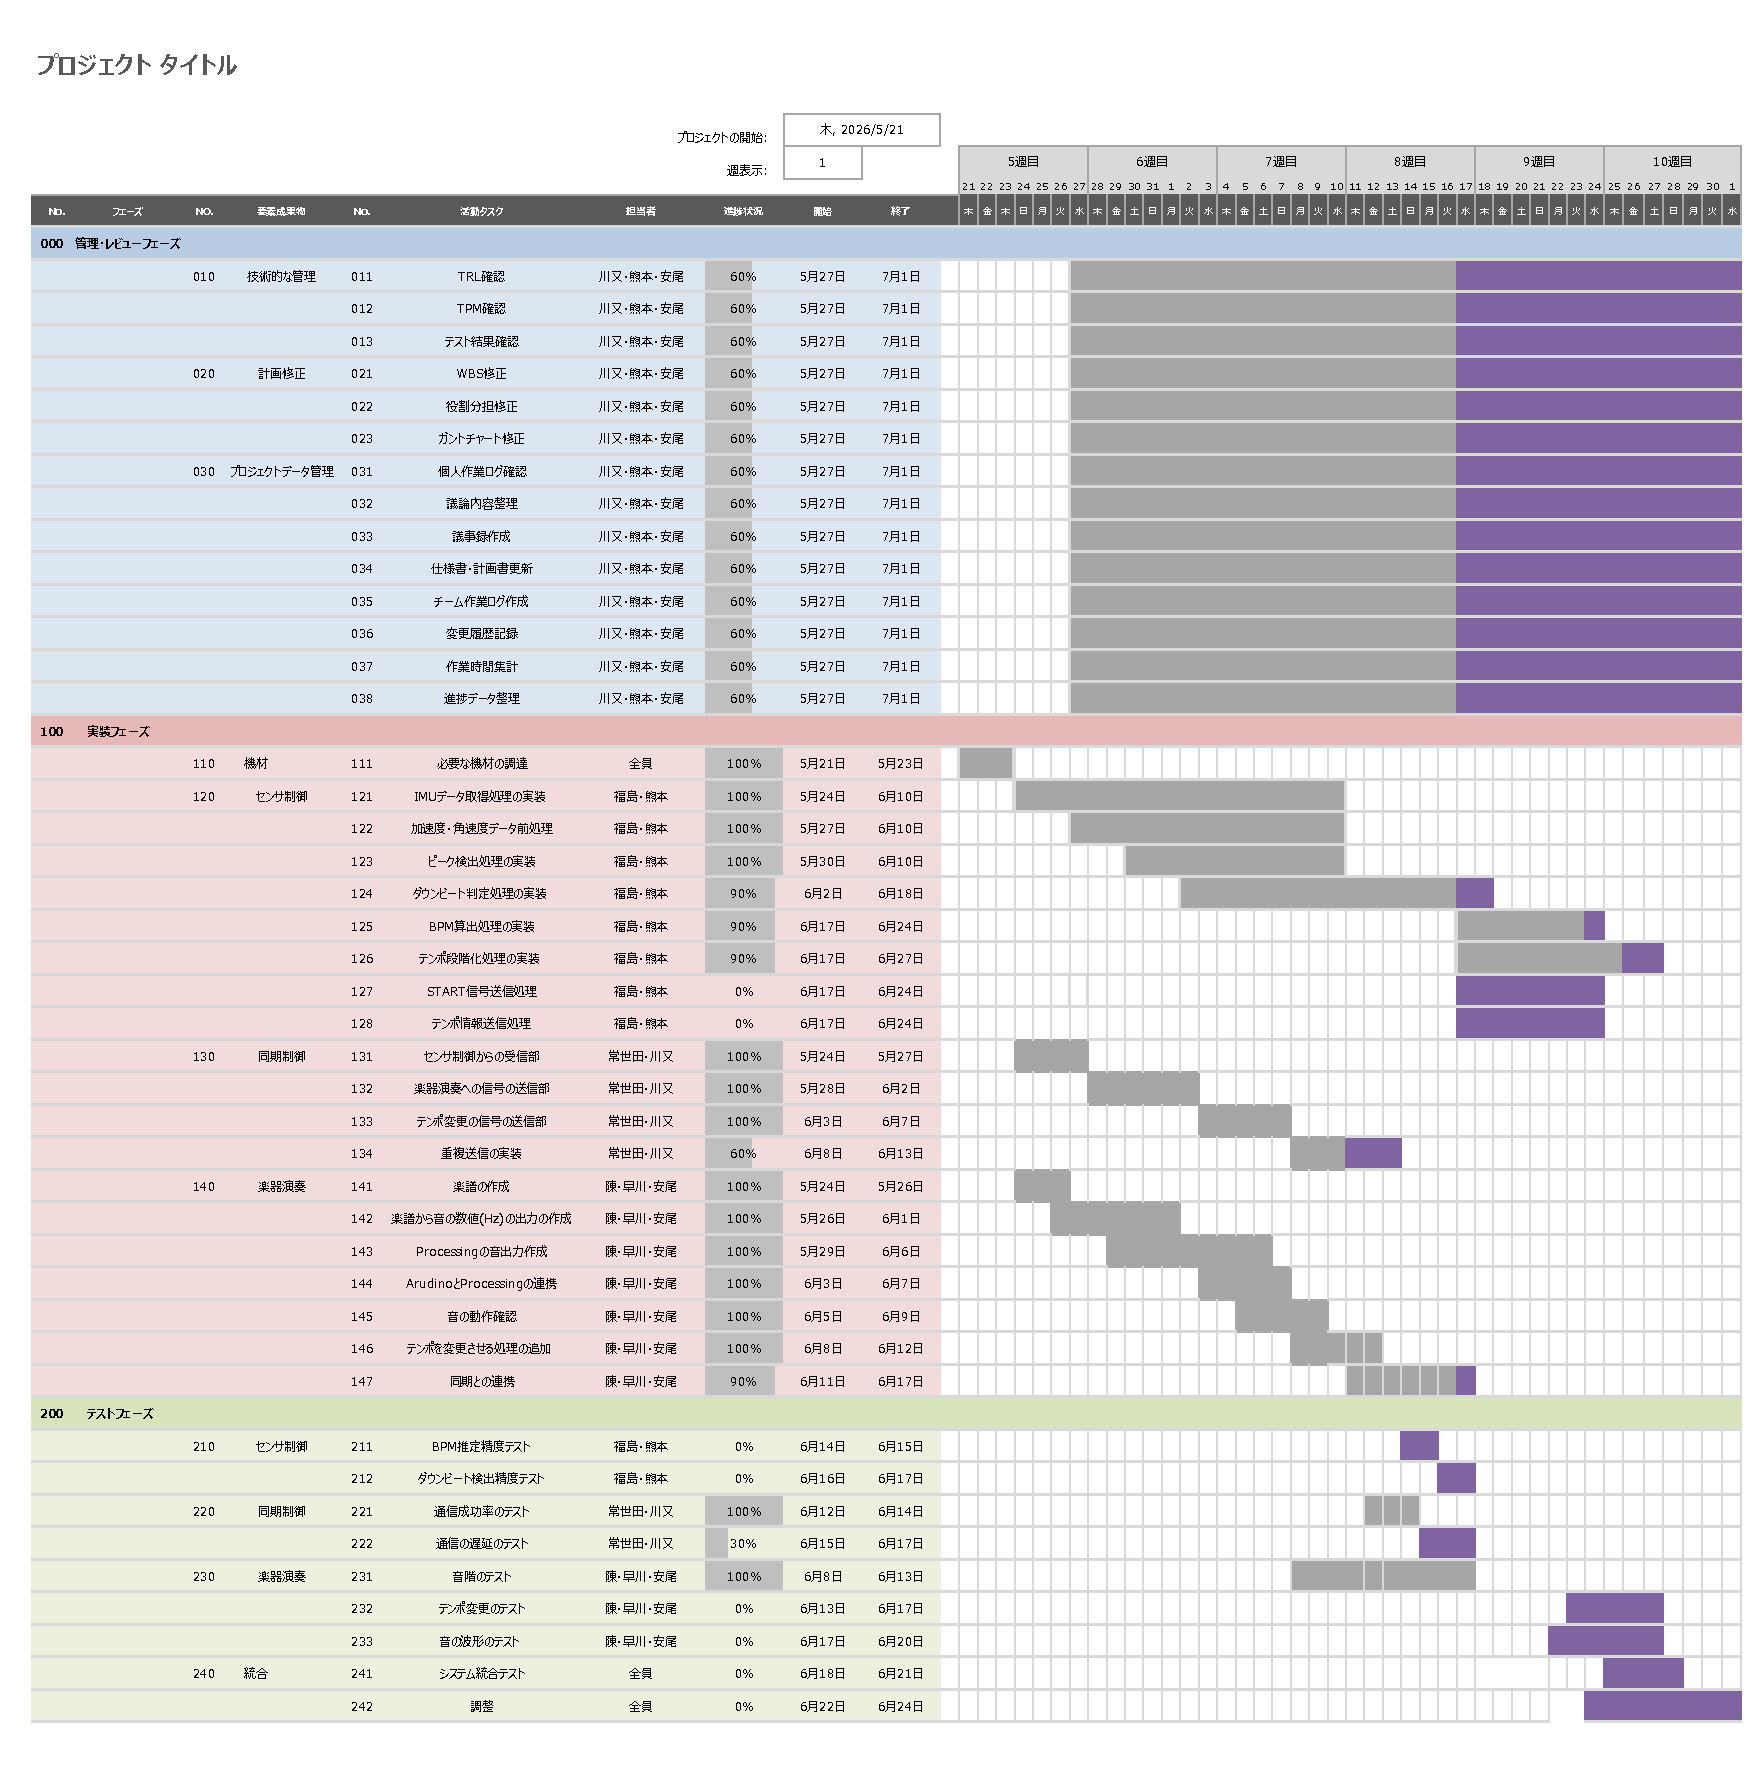
\includegraphics[width=0.8\textwidth]{gant8.pdf}
    \caption{ガントチャート}
\end{figure}

\section{日ごとの作業時間と作業内容}
今週実施した日ごとの具体的な作業時間および対応内容の詳細です．
\begin{table}[H]
    \centering
    \small
    \begin{tabular}{lll}
        \toprule
        日付 & 作業時間 & 作業内容 \\
        \midrule
        {}[6/24] & [2.0時間] & 制御用Arduinoと同期用Arduinoのコマンド連携の統合と動作確認． \\
        {}[6/27] & [2.0時間] & 楽器4台・サーボ・LEDマトリクスの統合と実機での輪唱動作確認． \\
        {}[6/30] & [2.0時間] & 音とLEDマトリクスの同期確認，および音ズレの測定． \\
        \midrule
        \textbf{合計} & \textbf{[6.0時間]} & \\
        \bottomrule
    \end{tabular}
\end{table}

\section{課題管理}
\begin{table}[H]
    \centering
    \small
    \begin{tabular}{p{3cm}p{3cm}llp{3cm}ll}
        \toprule
        課題 & 発生原因 & 影響度 & 優先度 & 対策 & 期限 & 状態 \\
        \midrule
        実機での通信遅延・音ズレ & 無線通信の遅延が合奏の同期精度に影響する可能性 & 中 & 高 & 実機で遅延を測定し，許容範囲に収まることを確認した & [6/30] & 解決 \\
        マトリクスと音の同期 & LEDアニメのコマ間隔とテンポ変更時の見た目のずれ & 低 & 低 & テンポに連動した表示間隔へ調整し，同期を確認した & [6/30] & 解決 \\
        \bottomrule
    \end{tabular}
\end{table}
\vspace{0.5em}
\noindent ※影響度=プロジェクトへのインパクト，優先度=対応の緊急性

\section{AI 利用状況と検証(再現性重視)}
\subsection{利用内容}
\begin{itemize}
    \item 利用目的: \LaTeX による作業ログのテンプレート作成
    \item  入力(プロンプト要旨):
    \begin{itemize}
        \item 指定された作業ログのテンプレート項目の生成を依頼 ．
    \end{itemize}
    \item  出力概要:
    \begin{itemize}
        \item テンプレートの構成のコンパイル可能な作業ログの\LaTeX ソースコード ．
    \end{itemize}
\end{itemize}

\subsection{検証方法}
\begin{itemize}
    \item  検証手法: 生成された\LaTeX ソースコードの構造確認およびコンパイル検証
    \item  参照資料: 提供された作業ログテンプレートPDF
    \item  検証手順:
    \begin{enumerate}
        \item 生成されたコードのセクション構成が，テンプレート項目を漏れなく満たしているか目視で確認．
        \item \LaTeX 環境において実際にコンパイルを行い，エラーを吐かずに正しくPDFが生成されるかを確認．
    \end{enumerate}
\end{itemize}

\section{その他}

\end{document}
